\section*{Câu 1 --- Hồi quy tuyến tính đơn}
Dữ liệu $(x_i,y_i)$: $(1,3),(2,5),(3,7),(4,9),(5,11)$, $n=5$, mô hình $y=\beta_0+\beta_1 x$.

\paragraph{(a)} Trung bình
\[
\bar x=\frac{1+2+3+4+5}{5}=3,\qquad
\bar y=\frac{3+5+7+9+11}{5}=7.
\]

\paragraph{(b)} Ta lập bảng $x_i-\bar x$, $y_i-\bar y$:
\begin{center}
\begin{tabular}{c|ccccc}
$x_i$ & 1 & 2 & 3 & 4 & 5 \\ \hline
$y_i$ & 3 & 5 & 7 & 9 & 11 \\
$x_i-\bar x$ & $-2$ & $-1$ & 0 & 1 & 2 \\
$y_i-\bar y$ & $-4$ & $-2$ & 0 & 2 & 4 \\
\end{tabular}
\end{center}
\[
SS_{xy}=\sum (x_i-\bar x)(y_i-\bar y)=(-2)(-4)+(-1)(-2)+0+1\cdot 2+2\cdot 4=8+2+2+8=20.
\]
\[
SS_x=\sum (x_i-\bar x)^2=4+1+0+1+4=10.
\]

\paragraph{(c)--(d)}
\[
\hat\beta_1=\frac{SS_{xy}}{SS_x}=\frac{20}{10}=2,\qquad
\hat\beta_0=\bar y-\hat\beta_1\bar x=7-2\cdot 3=1.
\]

\paragraph{(e)} Phương trình hồi quy: $\hat y=1+2x$.

\paragraph{(f)} Với $x=6$: $\hat y=1+2\cdot 6=13$.

\section*{Câu 2 --- Sai số \& MSE}
Cho $\hat y=2x+1$ và bộ mẫu $(1,4),(2,6),(3,8),(4,11)$, $n=4$.

\paragraph{(a)} $\hat y_1=3$, $\hat y_2=5$, $\hat y_3=7$, $\hat y_4=9$.

\paragraph{(b)} Đề định nghĩa $e_i=\hat y_i-y_i$:
\[
e_1=-1,\quad e_2=-1,\quad e_3=-1,\quad e_4=-2.
\]

\paragraph{(c)}
\[
MSE=\frac{1}{n}\sum_{i=1}^n e_i^2=\frac{1+1+1+4}{4}=\frac{7}{4}=1{,}75.
\]

\paragraph{(d)} MSE dương, có mẫu lệch khá hơn các mẫu còn lại ($|e_4|=2$); mô hình $\hat y=2x+1$ chưa khớp các quan sát $y$ của đề.

\section*{Câu 3 --- Một bước Gradient Descent}
Dữ liệu: $(1,3),(2,5),(4,9)$, $m=3$. Mô hình $\hat y=wx+b$, ban đầu $w=b=0$, $\eta=0{,}1$.
\[
J(w,b)=\frac{1}{2m}\sum_{i=1}^m (y_i-\hat y_i)^2.
\]
Đạo hàm (batch):
\[
\frac{\partial J}{\partial w}=-\frac{1}{m}\sum_{i}(y_i-\hat y_i)x_i,\qquad
\frac{\partial J}{\partial b}=-\frac{1}{m}\sum_{i}(y_i-\hat y_i).
\]
\paragraph{(a)} Với $w=b=0$ thì $\hat y_i=0$, nên $\hat y=(0,0,0)$.

\paragraph{(b)} $y-\hat y=(3,5,9)$:
\[
\frac{\partial J}{\partial w}=-\frac13(3\cdot 1+5\cdot 2+9\cdot 4)=-\frac{49}{3},\qquad
\frac{\partial J}{\partial b}=-\frac13(3+5+9)=-\frac{17}{3}.
\]

\paragraph{(c)}
\[
w\leftarrow w-\eta\frac{\partial J}{\partial w}=0+0{,}1\cdot\frac{49}{3}=\frac{49}{30},\qquad
b\leftarrow b-\eta\frac{\partial J}{\partial b}=0+0{,}1\cdot\frac{17}{3}=\frac{17}{30}.
\]

\paragraph{(d)} Sau một bước: $\hat y=\dfrac{49}{30}x+\dfrac{17}{30}$.

\section*{Câu 4 --- Hồi quy đa biến \& phương trình chuẩn}

\paragraph{(a)} Viết ma trận thiết kế có cột 1 cho hệ số tự do:
\[
X=\begin{bmatrix}
1&1&2\\1&2&1\\1&3&2\\1&4&3
\end{bmatrix},\qquad
Y=\begin{bmatrix}5\\6\\9\\12\end{bmatrix}.
\]

\paragraph{(b)} Phương trình chuẩn: $\hat\beta=(X^\top X)^{-1}X^\top Y$ với $\hat\beta=(\beta_0,\beta_1,\beta_2)^\top$.

\paragraph{(c)} Nhân trực tiếp cho
\[
X^\top X=\begin{bmatrix}4&10&8\\10&30&22\\8&22&18\end{bmatrix},\qquad
X^\top Y=\begin{bmatrix}32\\92\\70\end{bmatrix}.
\]

\paragraph{(d)--(e)} Giải hệ nhận $\hat\beta_0=1$, $\hat\beta_1=2$, $\hat\beta_2=1$.
Vậy $\hat y=1+2x_1+x_2$.

\paragraph{(f)} $(x_1,x_2)=(5,2)$:
\[
\hat y=1+2\cdot 5+2=13.
\]

\section*{Câu 5 --- Batch Gradient Descent (5 điểm)}
Dữ liệu $(x,y)$: $(1,2),(2,3),(3,5),(4,4),(5,6)$, $m=5$, $w^{(0)}=b^{(0)}=0$, $\eta=0{,}1$.
\[
\frac{\partial J}{\partial w}=-\frac15\sum_i (y_i-\hat y_i)x_i,\quad
\frac{\partial J}{\partial b}=-\frac15\sum_i (y_i-\hat y_i),\quad
J=\frac{1}{10}\sum_i (y_i-\hat y_i)^2.
\]
\paragraph{(a)} Tại $w=b=0$, $\hat y_i=0$ nên $\sum (y_i-\hat y_i)x_i = 2+6+15+16+30=69$ và $\sum (y_i-\hat y_i)=20$.
Do đó $\partial J/\partial w=-69/5$, $\partial J/\partial b=-4$, $J=\frac{1}{10}(4+9+25+16+36)=9$.

\paragraph{(b)} Một bước GD:
\[
w^{(1)}=0-0{,}1\cdot\Big(-\frac{69}{5}\Big)=1{,}38,\qquad
b^{(1)}=0-0{,}1\cdot(-4)=0{,}4.
\]

\paragraph{(c)} Dự báo $x=6$: $\hat y=1{,}38\cdot 6+0{,}4=8{,}68$.

\section*{Câu 6 --- Phân lớp đường ranh giới tuyến tính}
Cho $w=(2,-1)$, $b=1$: lớp 1 khi $2x_1-x_2+1\ge 0$, lớp 0 khi $<0$.
\begin{align*}
\text{A}(1{,}1){:}\quad &2-1+1=2 &&\text{(lớp 1)} \\
\text{B}(2{,}1){:}\quad &4-1+1=4 &&\text{(lớp 1)} \\
\text{C}(1{,}3){:}\quad &2-3+1=0 &&\text{(lớp 1)} \\
\text{D}(4{,}2){:}\quad &8-2+1=7 &&\text{(lớp 1)}.
\end{align*}
Theo đề điểm nằm trên đường có $w^\top x+b\ge 0$ thuộc lớp 1, nên cả A, B, C, D đều được gán \textbf{lớp 1}.

Đường ranh giới: $2x_1-x_2+1=0$, hay $x_2=2x_1+1$.

\begin{figure}[h]
   \centering
   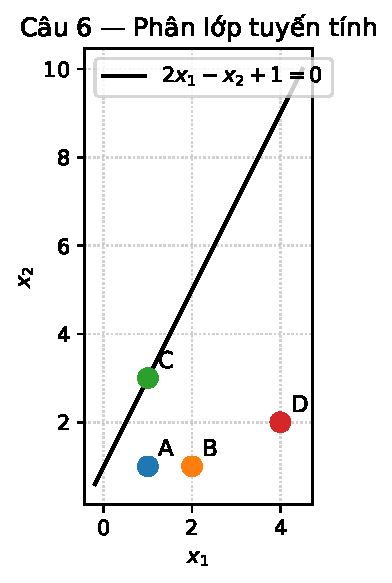
\includegraphics[width=0.62\linewidth]{figures/cau6_boundary.pdf}
   \caption{Các điểm và đường quyết định $2x_1-x_2+1=0$.}
\end{figure}

\section*{Câu 7 --- Logistic}
$z=0{,}5x_1-x_2+0{,}2$, $x=(2,1)$:
\[
z=0{,}5\cdot 2-1\cdot 1+0{,}2=0{,}2.
\]
\[
P(y=1\mid x)=\sigma(z)=\dfrac{1}{1+e^{-0{,}2}}\approx 0{,}5498.
\]
Ngưỡng $0{,}5$: $0{,}5498\ge 0{,}5$ $\Rightarrow$ lớp có nhãn dương ($y=1$).\\
Ngưỡng $0{,}8$: $0{,}5498<0{,}8$ $\Rightarrow$ lớp không dương ($y=0$).

\section*{Câu 8 --- Cross-entropy}

\paragraph{(a)} $L_i=-[y_i\ln z_i+(1-y_i)\ln(1-z_i)]$:
\[
L_1=-\ln 0{,}9,\quad L_2=-\ln 0{,}8,\quad L_3=-\ln 0{,}7.
\]

\paragraph{(b)} Tổng $J=L_1+L_2+L_3=-\ln(0{,}9\cdot 0{,}8\cdot 0{,}7)\approx 0{,}6852$.

\paragraph{(c)} Trung bình $\dfrac{J}{3}\approx 0{,}2284$.

\paragraph{(d)} Loss không quá lớn; mẫu 1 có xác suất dự báo gần nhãn 1 trong ba mẫu.

\section*{Câu 9 --- Perceptron (3 mẫu)}
Ba mẫu: $(1,1,t{=}1),(2,1,t{=}1),(1,3,t{=}{-}1)$; $\rho=1$, khởi tạo $w=(0{,}0)$, $b=0$.
Coi một mẫu \textbf{đã phân đúng} khi và chỉ khi $t_k(w^\top x_k+b)>0$.

\paragraph{(a)} Ban đầu $w^\top x_k+b=0$ với mọi k nên không mẫu nào thỏa bất đẳng thức nghiêm: cần các bước cập nhật trong PLA.

\paragraph{(b)--(c)} Một epoch, duyệt thứ tự mẫu 1\dots{}3; mỗi lần gặp mẫu không thỏa $t(w^\top x+b)>0$ thì
$w\leftarrow w+\rho\,t\,x$, $b\leftarrow b+\rho\,t$.
\begin{itemize}\itemsep0pt
    \item Mẫu 1 cần chỉnh $\Rightarrow$ sau cập nhật $(w,b)=((1,1),1)$;
    \item Mẫu 2 thỏa $t(w^\top x+b)=4>0$ $\Rightarrow$ giữ nguyên;
    \item Mẫu 3 thỏa điều kiện cập nhật $\Rightarrow$ $(w,b)=((0,-2),0)$.
\end{itemize}
Sau một epoch: $w=(0,-2)$, $b=0$.

\paragraph{(d)} Đường ranh giới $w^\top x+b=0$: $-2x_2=0$, tức $x_2=0$.

\section*{Câu 10 --- Hàm chi phí trên tập phân sai}
Dữ liệu $(x_1,x_2,t)$:
$(1,1,+1),(2,1,+1),(1,2,-1),(2,2,-1)$.
Khởi tạo $w=(1,1)$, $b=0$.
\[
J(w,b)=\sum_{k\in\mathcal Y}(-t_k)(w^\top x_k+b),\quad \mathcal Y=\{k: t_k(w^\top x_k+b)<0\}.
\]
Hai nhãn âm sai với dự đoán dương (độ lớn tuyến tính dương trên các mẫu đó).

\paragraph{(a)} $\mathcal Y=\{\text{mẫu 3 và 4}\}$.

\paragraph{(b)}
\[
\frac{\partial J}{\partial w}=\sum_{k\in\mathcal Y} (-t_k)\,x_k=(1{,}2)+(2{,}2)=(3{,}4),\qquad
\frac{\partial J}{\partial b}=\sum_{k\in\mathcal Y}(-t_k)=2.
\]
(Trình bày theo các thành phần tọa độ xuất hiện trong hàm tuyến tính trên các mẫu sai.)

\paragraph{(c)} Một bước học Rosenblatt với $\rho=1$ trên \textbf{mẫu sai đầu tiên} $(x{=}(1,2),\,t{=}{-}1)$:
\[
w^{(1)}=w^{(0)}+(-1)x=(0,-1),\quad b^{(1)}=b^{(0)}+(-1)=-1.
\]
